\scanpage{11}

$X$ surface topologique

$\mathcal G$ groupe discret opérant sur $X$

$G$ sous-groupe invariant de $\mathcal G$, opérant
proprement sur $X$, de sorte que \deleted{$\forall x\in X$}
\margin{\deleted{\illegible{1}}}
\inserted{\unsure{les}} stabilisateurs $G_x$ $(x\in X)$
\unsure{opèrent} fidèlement \unsure{au voisinage} de $x$, en
\unsure{conservant} l'orientation locale en $x$

$Y=X/G$ (surface topologique), $f\colon X\to Y$

$X^{!}$ \unsure{p.tie|partie} discrète de $X$, stable sous $\mathcal G$,

$d_X$ ``signature'' sur $X$ de support $X^{!}$, inv. par $\mathcal G$
\[
\unsure{i}\mapsto d_X(i)
\qquad X^{!}\longmapsto\mathbb N
\]

$Y^{!}\simeq X^{!}/G\subset Y$ \quad image de $X^{!}$ dans $Y$

On suppose $x\in X$, $G_x\ne\{1\}\ \Rightarrow\ x\in X^{!}$

\[
d_Y\colon Y^{!}\to\mathbb N,\qquad d_Y(y)=\nu_x d_X(x)
\]
\[
\text{si } y=f(x),\quad \nu_x=[G_x]
\]

$\mathrm{Rev}(X,d_X,\mathcal G)$ catégorie des $\mathcal G$-revêtements
ramifiés de $X$, \unsure{subordonnés} à $d_X$

$\mathrm{Rev}(Y,d_Y,\mathcal H)$ catégorie des $\mathcal H$-\unsure{revts}
ramifiés de $Y$, \unsure{subordonnés} à $d_Y$

Pour $X'\in\mathrm{Ob}\,\mathrm{Rev}(X,d_X,\mathcal G)$, considérons
$X'/G$ comme surface sur laquelle opère
$\mathcal H=\mathcal G/G$, au dessus de $Y=\unsure{X'/G|X/G}$. Alors

\margin{10}

\scanpage{12}
\mspage{294}

 a) $X'/G\in\mathrm{Ob}\,\mathrm{Rev}(Y,d_Y,\mathcal H)$

 b) On \unsure{trouve|donne} ainsi un foncteur
\[
\mathrm{Rev}(X,d_X,\mathcal G)\longrightarrow
\mathrm{Rev}(Y,d_Y,\mathcal H) \tag{19}
\]

 c) Ce foncteur est une équivalence de catégories.

 d) Description d'un foncteur quasi-inverse par image inverse ``normalisée''.

Remarques. OPS $d_X$ à valeurs $>0$ i.e. $d_Y$ à valeurs
$>0$ (sinon, si $S=\{x\in X^{!}\mid d_X(x)=0\}$, \unsure{remplaçons}
$X$ par $X\setminus S$), $Y$ par $Y\setminus T$ $(T=S/G)$.

\inserted{OPS $d_X(x)=1\ \Rightarrow\ [G_x]\ne1$
(sinon, \unsure{remplacer} $X^{!}$ \unsure{par} $X^{!}\setminus S$
$S=\{x\in X^{!}\mid d_X(x)=1,\ \unsure{[G_x]=1\}}$\unsure{)}}

Le cas le plus intéressant \unsure{pour nous est}
celui où \deleted{$d_X(x)=1$} $\forall x\in X^{!}$, \unsure{on a}
$d_X(\unsure{x})=1$ et $G_x\ne\{1\}$
(donc $X^{!}=\{x\in X\mid G_x\ne\{1\}\}$), \unsure{donc|dans} le cas où
\[
\mathrm{Rev}(X,d_X,\mathcal G)=\mathrm{Rev}(X,\mathcal G) \tag{20}
\]
et où $\mathrm{Rev}(\unsure{\deleted{\illegible{1}}}Y,d_Y,\mathcal H)$ peut donc
\unsure{s'interpréter} comme un $\mathrm{Rev}(X,\mathcal G)$
(sans \unsure{donnée} de ramification)

\margin{11}

\scanpage{13}

\uline{Corollaire} Soit $x\in X\setminus X^{!}$, $y$ son image dans
$Y\setminus Y^{!}$, on a un iso. canonique
\[
\Pi_1\bigl((X,d_X,\mathcal G)\unsure{,|;}x\bigr)
\overset{\sim}{\longrightarrow}
\Pi_1\bigl((Y,d_Y,\mathcal H)\unsure{,|;}y\bigr) \tag{21}
\]

Nous allons \unsure{expliciter} cet isomorphisme en termes de
\unsure{calculs} de \deleted{lacets}\inserted{chemins}.

Un élément\inserted{$\alpha$} de
$\Pi_1\bigl((X,d_X,\mathcal G)\unsure{,|;}x\bigr)$
% ``provient'': struck through, then restored by a row of dots under it (stet).
provient d'un couple $(\gamma,\ell)$, avec
\[
\gamma\in\mathcal G,\qquad
\ell\ \text{classe de chemins dans }X\setminus X^{!}
\text{ de }x\text{ vers }\gamma^{-1}x
\]

(\unsure{avec|car} $(\gamma,\ell)$ et $(\gamma',\ell')$ \unsure{définissent} le
$\overline{\mathrm m}$ élément, \unsure{ssi|sss} $\gamma'=\gamma$, et
\inserted{l'élément} $\ell'^{-1}\ell$ de $\Pi_1(X\setminus X^{!},x)$ est
dans le ss-groupe invariant noyau de
\[
\Pi_1(X\setminus X^{!},x)\longrightarrow\Pi_1((X,d_X),x)
\]
-- i.e. le ss-groupe invariant engendré par les
\deleted{\unsure{$k$|$\ell$}} $\lambda_a^{d_X(a)}$, où
pour tt $a\in X^{!}$, $\lambda_a$ désigne la \unsure{classe} dans
$\Pi_1(X\setminus X^{!},\unsure{x|a})$ d'un ``lacet de $x$ autour de $a$'').

Soit alors $\dot\gamma$ l'image de $\mathcal G$ dans $\mathcal H$ --
\deleted{\unsure{$f_0$|$f$}} soit
$f_U\colon X\setminus X^{!}\overset{\unsure{\mathrm{df}|\mathrm{def}}}{=}U
\longrightarrow Y\setminus Y^{!}\overset{\unsure{\mathrm{df}|\mathrm{def}}}{=}V
\simeq U/G$ l'\unsure{application}

\margin{12}

\scanpage{14}
\mspage{295}

canonique, alors l'image \inserted{$\beta$} de
\inserted{$\alpha\in\Pi_1(X,d_X,\mathcal G;x)$ \unsure{défini par}}
$(\gamma,\ell)$ \deleted{est}
dans $\Pi_1(Y,d_Y,\mathcal H;y)$ est $(\dot\gamma,f_U(\ell))$

(\uline{NB} $f_U(\ell)$ est une classe de \unsure{chemins} dans
$V=Y\setminus Y^!$ de $y=f_U(x)$ vers
$\dot\gamma^{-1}(y)=f_U(\gamma^{-1}x)$).

\inserted{\uline{NB.}} On voit tout de suite que si
$(\gamma,\ell)$ et $(\gamma',\ell')$ \unsure{définissent} un
$\overline{\mathrm m}$ $\alpha$, alors ils \unsure{définissent} aussi
un $\overline{\mathrm m}$ $\beta$, ce qui provient du fait que
\[
\Pi_1(f_U,a):\Pi_1(X\setminus X^!,x)
\longrightarrow\Pi_1(Y\setminus Y^!,y)
\]
applique un $\lambda_a$ dans \inserted{un} $\lambda_b^{\nu(a)}$
($b=f(a)$, $\nu(a)=[G_a]=$ degré de \unsure{ramification}
de $f$ en $a$) donc $\lambda_a^{d_X(a)}$ en
$\lambda_b^{d_X(a)\nu(a)=d_Y(b)}$.

Revenons à la situation de (13)
\[
X=U_{0,3}^{\mathrm{an}},\quad
\mathcal G=\mathcal T_{0,3}
=\mathfrak S_3\times\mathbb Z/2,\quad
G=\mathcal T_{0,3}^{+}
=\mathfrak S_3
\]
\margin{$X^!=\{\deleted{\illegible{1}}2,-1,\frac12;
-\bar j,\unsure{-j}\}$}
\[
Y\simeq\mathbb P^{1\,\mathrm{an}}\setminus\{0\},\quad
Y^!=\{1,\infty\},
\]
\inserted{$\mathcal H=\mathbb Z/2\mathbb Z$,}
application de \unsure{passage} au quotient de
$\widehat X=\mathbb P^{1\,\mathrm{an}}$ dans
$\widehat Y=\mathbb P^{1\,\mathrm{an}}$ donnée par (13)
\[
f(z)=\frac{3^3}{2^2}\frac{z^2(z-1)^2}{(z^2-z+1)^3}
\]
\margin{13}

\scanpage{15}

Pour calculer
$\Pi_1(Y,\underline{d}_Y,\mathbb Z/2\mathbb Z)
=\widetilde\Pi_{0,3}'$
(groupe carto-\unsure{graphique} \unsure{triangulé} non orienté),
on a pris le point base $y=-\bar j$, on va donc choisir
un $x\in\unsure{U_{0,3}^{\mathrm{an}}}$ au dessus de $y$, tel que
\[
f(x)=y=-\bar j
\]
--- il y a \deleted{six \unsure{places|points}} \inserted{un}
choix dans un \unsure{ens} $f^{-1}(\{y\})$ à six
éléments, dont \uline{trois} dans l'hémisphère nord
(les trois autres dans l'hémisphère sud),
ceux-ci sont permutés \unsure{transitivement} par $\rho$.
Ils se trouvent \unsure{respectivement} dans les
triangles sphériques $(-\bar j,0,\frac12)$, $(-\bar j,1,2)$,
$(-\bar j,\infty,-1)$ (appliqués par $f$
\unsure{homéomorphiquement} sur le triangle sphérique $(0,1,\infty)$
\unsure{supérieur}, \inserted{\unsure{dans l'hémisphère sup)}}
de centre $-\bar j$).
Le choix de $\unsure{x|a}$ \unsure{revient} donc
au choix de l'un des trois
\inserted{triangles sphériques, ou encore des 3}
segments sphériques $(0,\frac12)$, $(1,2)$, $(\infty,-1)$
--- j'ai envie de prendre $(0,\frac12)$, \unsure{correspondant}
au triangle $(-\bar j,0,\frac12)$.

Les trois générateurs \inserted{involutifs}
\deleted{\illegible{1}} $\tau'_0,\tau'_1,\tau'_\infty$
de $\Pi_1(Y,d_Y,
\unsure{\mathbb Z/2\mathbb Z|\mathbb Z/2})$
\unsure{au|en} dessus de $\tau\in\mathbb Z/2\mathbb Z$
s'obtiennent en prenant des chemins $\ell'_0,\ell'_1,\ell'_\infty$
de \inserted{\unsure{pôle nord}} $y=-\bar j$ vers
\inserted{\unsure{le pôle sud}} $\tau y=-j$, qui sont \unsure{les|des} arcs de
\unsure{grand cercle} coupant l'équateur resp. en $2,-1,\frac12$.

\margin{14}

\scanpage{16}
\mspage{296}

Ces chemins sont les images par $f$ de chemins
sur $X$, soient $\lambda_0:\overrightarrow{x,z_0}$,
$\inserted{\lambda_1:}\overrightarrow{x,z_1}$,
$\inserted{\lambda_\infty:}\overrightarrow{x,z_\infty}$,
qui coupent \inserted{chacun} la subdivision barycentrique du double
triangle sphérique $(0,1,\infty)$ en exactement un point,
\unsure{situé} \unsure{respectivement} sur le côté
$(\frac12,-\bar j)$, $(-\bar j,0)$ et $(0,\frac12)$
du triangle sphérique $(0,\frac12,-\bar j)$.

\margin{\uline{NB} Les points $z_0,z_1,z_\infty$
sont \unsure{caractérisés} \inserted{\unsure{resp$^{\mathrm t}$}}
comme les seuls points de $X$ au dessus de
$-j=f(\unsure{\dot\tau|\tau}x)$, se trouvant \unsure{ds|dans} les
triangles sphériques $(-\bar j,\frac12,1)$, $(0,-\bar j,-1)$,
$(\frac12,0,-j)$.}

Les points \deleted{\unsure{les}} $z_0,z_1,z_\infty$ au dessus de
$\tau y$ sont \unsure{respectivement} de la forme
$\inserted{g_0x=}\dot\sigma_\infty\dot\tau x$,
$\inserted{g_1x=}\dot\sigma_0\dot\tau x$,
$\inserted{g_\infty x=}\deleted{\unsure{\dot\sigma_\infty}}\dot\tau x$
\inserted{(i.e. $g_0=\dot\sigma_\infty\dot\tau$,
$g_1=\dot\sigma_0\dot\tau$, $g_\infty=\dot\tau$)}.
Ainsi les générateurs involutifs
$\tau'_0,\tau'_1,\tau'_\infty$ de
$\widetilde\Pi_{0,3}'=\Pi_1(Y,d_Y,\mathbb Z/2\mathbb Z;y)$
sont les images des éléments
\deleted{$(\dot\sigma_{\unsure{0}}\dot\tau,\lambda_0)$},
(notés par le $\overline{\mathrm m}$ signe)
\[
\tau'_0=(\dot\sigma_0\dot\tau,\lambda_0);\quad
\tau'_1=(\dot\sigma_1\dot\tau,\lambda_1),\quad
\tau'_\infty=(\dot\sigma_\infty\dot\tau,\lambda_\infty)
\]
de $\Pi_1(X,\mathcal G;x)$.
Nous allons utiliser l'arc de grand cercle \inserted{$\ell$}
de \deleted{$x=$} $-\bar j=P$
(\deleted{origine} \inserted{\unsure{point-base}}
\unsure{habituelle|habituel} \unsure{pour} le calcul de $\Pi_1(X,\mathcal G)$)
\inserted{à $x$}, pour identifier $\Pi_1(X,\mathcal G;x)$
à $\Pi_1(X,\mathcal G;P)$.

On peut alors prendre \deleted{\unsure{comme}}
\[
\tag{21}
\tau'_0=(\dot\sigma_0\dot\tau,\lambda'_0),\quad
\tau'_1=(\dot\sigma_1\dot\tau,\lambda'_1),\quad
\tau'_\infty=(\dot\sigma_\infty\dot\tau,\lambda'_\infty)
\]
où $\lambda'_0,\lambda'_1,\lambda'_\infty$ sont les
\deleted{arcs de grand cercle}
\inserted{\deleted{\unsure{lacets}} chemins de}
\deleted{(i.e. les \unsure{lacets|bouts} en $P$)}
de $P=-\bar j$
\inserted{vers \deleted{\illegible{1}} $\unsure{g_iP|\dot g_iP}$
\deleted{\illegible{1}}}
\deleted{vers $z_0,z_1,z_\infty$ \unsure{respectivement}
(qui, à l'excep-}

\margin{15}

\scanpage{17}

\deleted{tion du dernier, ne recoupent pas le graphe
barycentrique du double triangle sphérique
sauf en $P=-\bar j$, le dernier le recoupant
\inserted{\unsure{seul$^{\mathrm t}$}} en un
\deleted{seul} \unsure{autre} point, \unsure{situé} sur le segment
sphérique $(0,\frac12)$.}

\deleted{Les points $z_0,z_1,z_\infty$ sont \unsure{caractérisés}
\unsure{respectivement} comme les points $z$
tels que $f(z)=-j$, et qui se \unsure{trouvent} dans les
triangles sphériques $(\frac12,\unsure{-\bar j},1)$,
$(-\bar j,0,-1)$, $(0,\frac12,-j)$.}

\figure{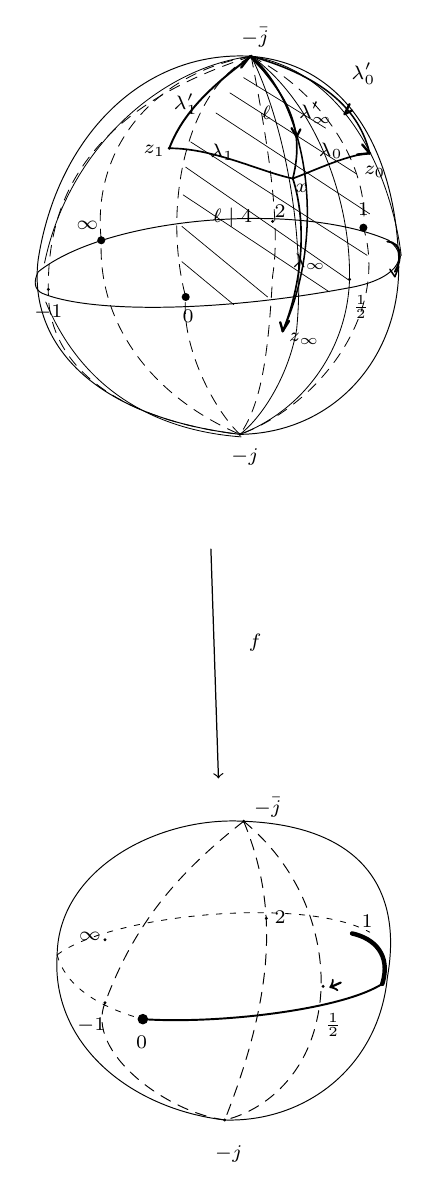
\begin{tikzpicture}[x=.016cm,y=-.016cm,line cap=round,line join=round,font=\scriptsize]
\coordinate (N) at (171,20);
\coordinate (S) at (162,320);
\coordinate (X) at (204,117);
\coordinate (Zone) at (106,93);
\coordinate (Zzero) at (265,97);
\coordinate (Zinf) at (196,238);
\draw[line width=.35pt] (N) .. controls (84,15) and (17,85) .. (2,181)
 .. controls (-6,243) and (39,305) .. (S)
 .. controls (236,319) and (290,260) .. (288,183)
 .. controls (286,105) and (253,27) .. (N);
\draw[line width=.3pt] (N) .. controls (99,29) and (26,93) .. (7,184);
\draw[line width=.3pt] (8,215) .. controls (38,287) and (97,317) .. (163,322);
\draw[line width=.3pt] (N) .. controls (250,33) and (283,121) .. (290,178);
\draw[line width=.35pt] (2,191) .. controls (57,147) and (209,135) .. (280,166)
 .. controls (299,180) and (284,198) .. (247,204)
 .. controls (145,223) and (43,224) .. (5,208)
 .. controls (-1,205) and (-2,199) .. (2,191);
\draw[dash pattern=on 4pt off 3pt,line width=.3pt] (N)
 .. controls (95,33) and (44,92) .. (52,166)
 .. controls (49,232) and (92,290) .. (S);
\draw[dash pattern=on 4pt off 3pt,line width=.3pt] (N)
 .. controls (117,49) and (101,143) .. (119,211)
 .. controls (115,248) and (140,299) .. (S);
\draw[dash pattern=on 4pt off 3pt,line width=.3pt] (N)
 .. controls (183,84) and (195,151) .. (188,194)
 .. controls (185,246) and (181,294) .. (S);
\draw[dash pattern=on 4pt off 3pt,line width=.3pt] (N)
 .. controls (230,50) and (265,110) .. (260,156)
 .. controls (281,225) and (223,298) .. (S);
\draw[dash pattern=on 4pt off 3pt,line width=.3pt] (N)
 .. controls (54,58) and (9,121) .. (10,205)
 .. controls (9,264) and (62,308) .. (S);
\draw[line width=.3pt] (N) .. controls (219,54) and (250,129) .. (249,197)
 .. controls (247,257) and (208,303) .. (S);
\draw[line width=.3pt] (N) .. controls (199,77) and (214,166) .. (207,237)
 .. controls (200,276) and (178,308) .. (S);
\draw[line width=.25pt] (165,37)--(230,77)
 (154,49)--(254,113) (143,65)--(265,145)
 (123,88)--(263,178) (119,108)--(249,198)
 (117,130)--(233,207) (116,155)--(184,211)
 (116,183)--(157,217);
\draw[line width=.7pt] (Zone) .. controls (118,61) and (146,39) .. (N);
\draw[line width=.6pt] (Zone) .. controls (142,93) and (179,112) .. (X);
\draw[line width=.6pt] (X) .. controls (225,109) and (248,98) .. (Zzero);
\draw[line width=.6pt] (X) .. controls (217,158) and (209,207) .. (Zinf);
\draw[line width=.6pt] (N) .. controls (196,49) and (215,73) .. (X);
\draw[line width=.55pt] (N) .. controls (231,37) and (257,64) .. (Zzero);
\draw[line width=.55pt] (N) .. controls (215,58) and (232,159) .. (Zinf);
\draw[line width=.85pt] (163,29)--(170,20)--(181,31);
\draw[line width=.85pt] (259,90)--(265,97)--(255,98);
\draw[line width=.85pt] (201,230)--(196,238)--(194,231);
\draw[line width=.85pt] (249,58)--(245,66)--(251,63);
\draw[line width=.8pt] (203,77)--(207,84)--(210,78);
\draw[line width=.7pt] (279,167) .. controls (291,168) and (291,181) .. (285,191);
\draw[line width=.55pt] (281,189)--(285,195)--(288,187);
\foreach \p in {(171,20),(162,320),(204,117),(106,93),(265,97),(196,238),(10,205),(249,197),(188,151)}
  \fill \p circle[radius=1.3];
\foreach \p in {(52,166),(119,211),(260,156)}
  \fill \p circle[radius=3.2];
\node[inner sep=0pt] at (174,5) {$-\bar j$};
\node[inner sep=0pt] at (166,338) {$-j$};
\node[inner sep=0pt] at (41,154) {$\infty$};
\node[inner sep=0pt] at (194,143) {$2$};
\node[inner sep=0pt] at (260,141) {$1$};
\node[inner sep=0pt] at (10,223) {$-1$};
\node[inner sep=0pt] at (121,226) {$0$};
\node[inner sep=0pt] at (258,219) {$\frac12$};
\node[inner sep=0pt] at (211,125) {$x$};
\node[inner sep=0pt] at (94,95) {$z_1$};
\node[inner sep=0pt] at (269,112) {$z_0$};
\node[inner sep=0pt] at (213,244) {$z_\infty$};
\node[inner sep=0pt] at (148,96) {$\unsure{\lambda_1}$};
\node[inner sep=0pt] at (234,95) {$\lambda_0$};
\node[inner sep=0pt] at (217,183) {$\unsure{\lambda_\infty}$};
\node[inner sep=0pt] at (119,58) {$\unsure{\lambda'_1}$};
\node[inner sep=0pt] at (260,34) {$\lambda'_0$};
\node[inner sep=0pt] at (222,65) {$\unsure{\lambda'_\infty}$};
\node[inner sep=0pt] at (183,65) {$\unsure{\ell}$};
\node[inner sep=0pt] at (156,148) {$\unsure{\ell\mid4}$};
\draw[->,line width=.45pt] (139,411)--(145,593);
\node[inner sep=0pt] at (174,485) {$f$};
\coordinate (NN) at (165,627);
\coordinate (SS) at (150,864);
\draw[line width=.35pt] (NN) .. controls (97,623) and (18,665) .. (17,733)
 .. controls (12,803) and (74,855) .. (SS)
 .. controls (214,866) and (272,822) .. (279,751)
 .. controls (293,672) and (249,630) .. (NN);
\draw[dash pattern=on 4pt off 3pt,line width=.35pt] (NN)
 .. controls (106,673) and (76,715) .. (55,771)
 .. controls (39,810) and (104,858) .. (SS);
\draw[dash pattern=on 4pt off 3pt,line width=.35pt] (NN)
 .. controls (190,688) and (193,755) .. (SS);
\draw[dash pattern=on 4pt off 3pt,line width=.35pt] (NN)
 .. controls (220,672) and (234,739) .. (223,785)
 .. controls (213,831) and (180,857) .. (SS);
\draw[dash pattern=on 2pt off 3pt,line width=.3pt] (17,733)
 .. controls (59,701) and (213,686) .. (265,715);
\draw[dash pattern=on 2pt off 3pt,line width=.3pt] (17,733)
 .. controls (24,759) and (52,775) .. (85,784);
\draw[line width=.7pt] (85,784)
 .. controls (143,788) and (242,777) .. (275,756);
\draw[line width=1.6pt] (251,716)
 .. controls (269,720) and (282,733) .. (275,756);
\draw[->,line width=.8pt] (242,755)--(233,759);
\foreach \p in {(165,627),(150,864),(55,721),(55,771),(183,704),(228,758)}
  \fill \p circle[radius=1.3];
\fill (85,784) circle[radius=4.2];
\node[inner sep=0pt] at (184,616) {$-\bar j$};
\node[inner sep=0pt] at (153,891) {$-j$};
\node[inner sep=0pt] at (43,718) {$\infty$};
\node[inner sep=0pt] at (44,789) {$-1$};
\node[inner sep=0pt] at (84,802) {$0$};
\node[inner sep=0pt] at (236,789) {$\frac12$};
\node[inner sep=0pt] at (263,706) {$1$};
\node[inner sep=0pt] at (194,703) {$2$};
\end{tikzpicture}}

\unsure{donnés} par
\[
\lambda'_i=\bigl(\deleted{\unsure{\tau_i\mid\ell_i}}\dot g_i(\ell^{-1})\bigr)(\lambda_i)\ell.
\]

On a donc
\[
\lambda'_0=
\underbrace{(\dot\sigma_\infty\dot\tau)}_{
\substack{\text{symétrie}\\
\text{p.r. au}\ \deleted{\text{l'équa}}\\
\unsure{\text{plan}}\ (\infty,-\bar j,\frac12,-j)}}
(\ell^{-1})\circ\lambda_0\circ\ell
\]
\inserted{\unsure{tous|est}} homotope au lacet trivial dans
$U_{0,3}$

\[
\lambda'_1=
\underbrace{\dot\sigma_0\dot\tau}_{
\substack{\text{symétrie}\\
\unsure{\text{p.r. à}}\ \text{l'équateur}\\
(0,-\bar j,2,-j)}}
(\ell^{-1})\circ\lambda_1\circ\ell
\]
homotope au lacet trivial dans $U_{0,3}$

\[
\lambda'_\infty=(\underbrace{\tau}(\ell^{-1}))\circ\lambda_\infty\circ\ell
\]
homotope au \deleted{chemin} \inserted{arc de}
grand cercle $(-\bar j,\frac12,-j)$
de $P=\unsure{-\bar j|\bar j}$ vers $\dot\tau P=-j$

\margin{16}

\scanpage{18}
\mspage{297}

En résumé, \unsure{avec} les notations de [C] \deleted{(13)} p.~7 \unsure{ff}, on aura donc
\[
\left\{
\begin{aligned}
\tau'_0&=\widetilde{\sigma}_\infty &&(\text{sur }\dot{\sigma}_\infty\dot{\tau})\\
\tau'_1&=\widetilde{\sigma}_0 &&(\text{sur }\dot{\sigma}_0\dot{\tau})\\
\tau'_\infty&=\tau_\infty &&(\text{sur }\dot{\tau})
\end{aligned}
\right.
\tag{22}
\]
\margin{NB $\tau_\infty=\sigma_\infty\widetilde{\sigma}_\infty=\widetilde{\sigma}_\infty\sigma_\infty$}

Il faut vérifier les relations essentielles
\[
\tau_0^{\prime\,2}=\tau_1^{\prime\,2}=\tau_\infty^{\prime\,2}
=\bigl(\underbrace{\tau'_0\tau'_\infty}_{\sigma_\infty}\bigr)^2
=\bigl(\underbrace{\tau'_1\tau'_0}_{\rho^{-1}}\bigr)^3=1
\tag{23}
\]
les quatre premières sont claires, la dernière s'écrit
\[
(\widetilde{\sigma}_0\widetilde{\sigma}_\infty)^3=1
\]
or on a
\[
\widetilde{\sigma}_0\widetilde{\sigma}_\infty=\rho^{-1}
\qquad (\inserted{[C],}\ \text{formule 13,})
\]
d'où ce qu'on veut.

Calculons (\unsure{conformément} à (18)) $\tau'_\infty\tau'_1$, $\tau'_0\tau'_\infty$, $\underbrace{\tau'_1\tau'_0}_{\rho^{-1}}$ --- qui \unsure{devront correspondre} à $\ell'_0,\ell'_1,\ell'_\infty$ ---
\[
\begin{aligned}
\ell'_0&=\tau'_\infty\tau'_1=\tau_\infty\widetilde{\sigma}_0
=\sigma_\infty\underbrace{\widetilde{\sigma}_\infty\widetilde{\sigma}_0}_{\rho}
=\sigma_\infty\rho\\
\ell'_1&=\tau'_0\tau'_\infty=\sigma_\infty\\
\ell'_\infty&=\tau'_1\tau'_0=\rho^{-1}
\end{aligned}
\]
i.e.
\[
\ell'_0=\sigma_\infty\rho,\quad \ell'_1=\sigma_\infty,\quad \ell'_\infty=\rho^{-1}
\tag{24}
\]
avec les relations caractéristiques
\[
\ell'_\infty\ell'_1\ell'_0=1,\qquad \ell_{\unsure{1|\infty}}^{\prime\,2}=1,\qquad \ell_\infty^{\prime\,3}=1
\tag{25}
\]
Tout est OK !

\margin{On exprime les éléments remarquables $\rho,\sigma_0,\sigma_1,\sigma_\infty,\ell_0,\ell_1,\ell_\infty,\tau_0,\tau_1,\tau_\infty$ de $\Pi_1(U_{0,3}^{\mathrm{an}};\mathfrak S_3\times\mathbb Z/2)$ en fonction des $\tau'_0,\tau'_1,\tau'_\infty$ ainsi :
\[
\begin{aligned}
\rho&=\tau'_0\tau'_1\\
\tau_\infty&=\tau'_\infty,\quad
\tau_0=\rho\tau_\infty\rho^{-1}=\tau'_0\tau'_1\tau'_\infty\tau'_1\tau'_0,\\
\tau_1&=\rho^{-1}\tau_\infty\rho=\ldots=\tau'_1\tau'_\infty\tau'_1
\end{aligned}
\]
\inserted{\unsure{$=\tau'_\infty\tau'_0$}}
\[
\begin{aligned}
\sigma_\infty&=\tau'_0\tau'_\infty,\quad
\sigma_0=\rho\sigma_\infty\rho^{-1}=\tau'_0\tau'_1\tau'_0\tau'_\infty\unsure{\tau'_1\tau'_0},\\
\sigma_1&=\rho^{-1}\sigma_\infty\rho=\tau'_1\tau'_\infty\tau'_0\tau'_1\\
\ell_0&=\tau_\infty\tau_1=\tau'_\infty\tau'_1\tau'_\infty\tau'_1=(\tau'_\infty\tau'_1)^2\\
\ell_1&=\tau_0\tau_\infty=\tau'_0\tau'_1\tau'_\infty\tau'_1\tau'_0\unsure{\tau'_\infty}\\
\ell_\infty&=\tau_1\tau_0=(\underbrace{\tau'_1\tau'_\infty\tau'_1}\tau'_0)^2
\end{aligned}
\]
\[
\begin{aligned}
\varepsilon_0&=\ell'_0=\deleted{\unsure{\tau'_1\tau'_\infty}}\unsure{\tau'_\infty\tau'_1}\\
\varepsilon_1&=\unsure{\tau'_0\tau'_1\tau'_\infty\tau'_0}\\
\varepsilon_\infty&=\tau'_1\tau'_\infty\tau'_1\unsure{\tau'_0}
\end{aligned}
\]
}
\margin{17}

\scanpage{19}

Je voudrais encore expliciter la \unsure{relation} de
$\widetilde{\Pi}'_{0,3}$ \inserted{gr. \unsure{carto-graphique} non orienté}
$\simeq\mathfrak S_{0,3}$ \inserted{$=\mathrm{Aut}_{\unsure{\mathrm{loc}|\mathrm{ext}}}(\Pi_{0,3})$}
avec $\mathrm{GP}(1,\mathbb Z)\simeq\mathrm{Gl}(2,\mathbb Z)'\overset{\mathrm{def}}{=}\mathrm{Gl}(2,\mathbb Z)/\{\pm1\}$.
Rappelons d'abord l'opération de
\[
\mathrm{GP}(1,\mathbb R)\simeq\mathrm{Gl}(2,\mathbb R)/\mathbb R^*
\simeq\mathrm{Gl}(2,\mathbb R)^{\pm1}/\{\pm1\}\quad\deleted{\unsure{\mathrm{GP}(|\text{agit}}}
\tag{26}
\]
sur le demi-plan de Poincaré $D$
\[
D=\{z\in\mathbb C\mid\Im(z)>0\}=\{x+iy\mid x\in\mathbb R,y\in\mathbb R^{*+}\}.
\tag{27}
\]
On fait opérer la matrice $u=\begin{pmatrix}a&b\\c&d\end{pmatrix}$ par
\[
f_u(z)=\left\{\begin{array}{ll}
\dfrac{az+b}{cz+d}&\text{si }\det u>0\\[4pt]
\dfrac{a\bar z+b}{c\bar z+d}&\text{si }\det u<0
\end{array}\right.
\tag{28}
\]
De cette façon, $\mathrm{GP}(1,\mathbb R)$ est isomorphe au groupe des automorphismes \uline{conformes} de $D$.

\margin{\uline{NB} $\mathrm{GP}(1,\mathbb R)$ a deux \unsure{comp. connexes}. \unsure{Sa comp. neutre} \inserted{$\mathrm{GP}(1,\mathbb R)^+$} est l'image de $\mathrm{Sl}(2,\mathbb R)$ (\unsure{ou de|de} $\mathrm{Gl}(2,\mathbb R)^+$) et s'identifie à $\mathrm{Sl}(2,\mathbb R)/\pm1$.}

D'ailleurs, la donnée d'une courbe elliptique \inserted{$E$} sur $\mathbb C$ équivaut à celle d'un espace $V$ de dim 1 sur $\mathbb C$, et d'un ``réseau'' $\pi\subset V$ (sous-groupe discret de rg 2).
\margin{équivalence de catégories \illegible{1}.}
L'orientation canonique de $V$ correspond à un générateur \unsure{$\eta|\gamma$} de $\bigwedge^2_{\mathbb Z}\pi$ --- ainsi $\pi$ est ``orienté''. Le choix d'une rigidification
\margin{18}

\scanpage{20}
\mspage{298}

de Jacobi unimodulaire de $\pi$, équivaut à celui d'une base $(e_1,e_2)$ de $\pi$ \inserted{(comme $\mathbb Z$-module)} telle que $e_1\wedge e_2=\unsure{\eta|\gamma}$. L'élément $e_1$ \inserted{(comme base de $V$ sur $\mathbb C$)} permet d'ailleurs d'identifier $V$ à $\mathbb C$, $e_1$ devenant 1. Ainsi la donnée de $E$ avec sa rigidification de Jacobi unimodulaire, équivaut à celle d'un élément $e_2=\tau$ de $\unsure{\mathbb C|E}$, tel que

\uline{1\textsuperscript{o}}) $(1,\tau)$ \unsure{engendrent|engendre} un sous-groupe discret de rg 1, i.e. $\tau\notin\mathbb R$ i.e. $\Im\tau\ne0$

2\textsuperscript{o}) l'orientation dudit sous-groupe définie par la base $(1,\tau)$ est ``directe'', i.e. $\Im\tau>0$, i.e. $\tau\in D$.

Quand on regarde l'opération de $\mathrm{Sl}(2,\mathbb Z)$ sur \inserted{l'ens} des classes d'isomorphie des courbes ell. rigidifiées, \unsure{ens.} \unsure{identifié} à $D$, on trouve que $\begin{pmatrix}a,b\\c,d\end{pmatrix}$ opère par $\tau\longmapsto\dfrac{a\tau+b}{c\tau+d}$, i.e. c'est l'opération naturelle de $\mathrm{Sl}(2,\mathbb Z)$ sur $D$, à travers $\mathrm{Sl}(2,\mathbb Z)'\simeq\mathrm{GP}(1,\mathbb Z)^+$.

Ce groupe opère proprement, Il a exactement deux trajectoires critiques, qui corres-
\margin{19}
